\chapter{Stand der Technik}
\label{chapter:Stand_der_Technik}
\myboxy{
	\begin{itemize}
		\item Bilder neu machen aus dem Schaltplan.
		\item Vector Controller, Funktionsweise nur kurz erklären und mehr auf die Anschlüsse eingehen.
		\item PIN-Mapping als Tabelle erstellen, für den Motor und den Vector Controller.
		\item QElectroTeck.
		\item PIN-Mapping als Tabelle erstellen, für den Motor und den Vector Controller.
		\item Auf die PDF verweisen.
	\end{itemize}
}{To-do}{\textwidth}



Im folgenden Abschnitt werden die verwendeten Bauteile, welche in Kapitel \ref{chapter:Konzept} dargestellt worden sind, näher beschrieben.


\section{Antrieb – Golden Motor}
\label{section:Antrieb}

Golden Motor bietet eine Gesamtlösung bestehend aus einem BLDC-Motor und einem Vektor-Controller an. Der Controller besitzt eine Schnittstelle für alle notwendigen Steuer- und Kontrollsignale, um den Motor anzutreiben. Die Anschlüsse sowie die grundlegende Funktionsweise werden in den Abschnitten \ref{section:BLDC_Motor} und \ref{section:Vector_Controller} näher erläutert.



\subsection{BLDC Motor}
\label{section:BLDC_Motor}

Der in Abbildung \ref{BLDC_Motor:img:antrieb_motor} dargestellte BLDC-Motor verfügt über eine Leistung von 10 kW und kann optional durch eine Ölkühlung gekühlt werden, was jedoch für das Fahrzeug derzeit nicht relevant ist. Die Drehzahl ist variabel und kann, mittls des Vector Controllers, welcher in Abschnitt \ref{section:Vector_Controller} erklärt wird, zwischen 2.000 und 6.000 U/min eingestellt werden. Das Nenndrehmoment beträgt 26 Nm, während das maximale Drehmoment bei 85 Nm liegt. Der Wirkungsgrad des Motors beträgt 91 \% \cite{Golden_Motor:bldc_motor}.

\pagebreak[1]
\begin{figure}[!ht]
	\begin{center}
		\includegraphics[width=1\textwidth]{img/2_antrieb/motor_1.png}
		\caption{Golden Motor – 10 KW BLDC Motor Liquid Cooled}
		\label{BLDC_Motor:img:antrieb_motor}
	\end{center}
\end{figure}


Die Anschlüsse des Motors sind in Tabelle \ref{BLDC_Motor:tab:pinmapping} aufgelistet. Der Motor verfügt über zwei Hall-Sensor-Kabel, die jeweils drei Hall-Sensoren sowie einen Temperatursensor enthalten. Zusätzlich sind ein GND- und ein +5V-Versorgungsanschluss in den Hall-Sensor-Kabeln integriert. Die Spulen des Motors werden über sechs separate Kabel angeschlossen: U, V und W.
\pagebreak[1]
\begin{table}[!ht]
	\centering
	\caption{Pin Mapping – BLDC-Motor}
	\label{BLDC_Motor:tab:pinmapping}
	\begin{tabular}{lll}
		\hline
		\textbf{Anschluss}          & \textbf{Funktionalität} & \textbf{Farbe} \\ \hline
		\multicolumn{3}{c}{\textbf{Anschluss Adern Motor}}                     \\ \hline
		\multicolumn{1}{l|}{U1}     & Spule 1                 & Gelb           \\
		\multicolumn{1}{l|}{V1}     & Spule 2                 & Grün           \\
		\multicolumn{1}{l|}{W1}     & Spule 3                 & Blau           \\
		\multicolumn{1}{l|}{U2}     & Spule 1                 & Gelb           \\
		\multicolumn{1}{l|}{V2}     & Spule 2                 & Grün           \\
		\multicolumn{1}{l|}{W2}     & Spule 3                 & Blau           \\ \hline
		\multicolumn{3}{c}{\textbf{Motor Hall Kabel 1}}                        \\ \hline
		\multicolumn{1}{l|}{Hall A} & Hall Sensor             & Gelb           \\
		\multicolumn{1}{l|}{Hall B} & Hall Sensor             & Grün           \\
		\multicolumn{1}{l|}{Hall C} & Hall Sensor             & Blau           \\
		\multicolumn{1}{l|}{Temp}   & Temperatur Sensor       & Weiß           \\
		\multicolumn{1}{l|}{+5V}    & Spannungsversorgung     & Rot            \\
		\multicolumn{1}{l|}{GND}    & Masse                   & Schwarz        \\ \hline
		\multicolumn{3}{c}{\textbf{Motor Hall Kabel 2}}                        \\ \hline
		\multicolumn{1}{l|}{Hall A} & Hall Sensor             & Gelb           \\
		\multicolumn{1}{l|}{Hall B} & Hall Sensor             & Grün           \\
		\multicolumn{1}{l|}{Hall C} & Hall Sensor             & Blau           \\
		\multicolumn{1}{l|}{Temp}   & Temperatur Sensor       & Weiß           \\
		\multicolumn{1}{l|}{+5V}    & Spannungsversorgung     & Rot            \\
		\multicolumn{1}{l|}{GND}    & Masse                   & Schwarz        \\ \hline
	\end{tabular}
\end{table}
\pagebreak[4]



\subsubsection{Funktionsweise}
\label{BLDC_Motor:Funktionsweise}
Ein BLDC-Motor (Brushless DC Motor) unterscheidet sich grundlegend von einem herkömmlichen Gleichstrommotor. Während bei einem traditionellen DC-Motor die Polumschaltung (Kommutierung) mechanisch über Kohlebürsten erfolgt, übernimmt beim BLDC-Motor eine elektronische Steuerung diese Aufgabe. Dadurch entfällt die Notwendigkeit von Kohlebürsten, was den Motor effizienter und langlebiger macht\cite{mathworks:bldc_motor}.
\newpage



\subsection{Vector Controller}
\label{section:Vector_Controller}

Der Motor wird mithilfe eines Vektor-Controllers angesteuert, der in Abbildung \ref{Vector_Controller:img:Antrieb_Controller} dargestellt ist. Der Controller hat die Aufgabe, den Motor basierend auf den Eingangssignalen so zu steuern, dass beispielsweise eine gewünschte Drehzahl erreicht wird. Die genaue Funktionsweise des Vektor-Controllers wird kurz unter \ref{Vector_Controller:Funktionsweise} erläutert.

Das Pin-Mapping ist in Tabelle \ref{Vector_Controller:tab:pinmapping} aufgeführt. Bei den Steuersignalen muss auf den Spannungsbereich geachtet werden, da der Controller eine Störung meldet, wenn ein Signal außerhalb des zulässigen Bereichs liegt. Dies ist ein integriertes Sicherheitssystem des Controllers. Dies ist ein integriertes Sicherheitssystem des Controllers. So liegt beispielsweise bei der Bremse das logische Signal bei 0, wenn die Spannung 1 V beträgt. Tritt ein Kabelbruch ein, wird die Spannung am Controller bei 0 V liegen und eine Warnung wird durch ein periodisches Tonsignal ausgegeben.


\begin{figure}[!ht]
	\begin{center}
		\includegraphics[width=1\textwidth]{img/2_antrieb/sine_1.png}
		\caption{Golden Motor – VECTOR 500 Motor Controller}
		\label{Vector_Controller:img:Antrieb_Controller}
	\end{center}
\end{figure}

\begin{table}[!ht]
	\centering
	\caption{Pin Mapping – Vector Controller}
	\label{Vector_Controller:tab:pinmapping}
	\begin{tabular}{lll|l}
		\hline
		\textbf{Anschluss}           & \textbf{Funktionalität}  & \textbf{Farbe}              & \textbf{U in V}                  \\ \hline
		\multicolumn{4}{c}{\textbf{Batterie Eingang}}                                                                            \\ \hline
		\multicolumn{1}{l|}{B+}      & Versorgungsspannung      & RT                          & 48 V                             \\
		\multicolumn{1}{l|}{B-}      & Masse                    & SW                          & 0 V                              \\ \hline
		\multicolumn{4}{c}{\textbf{Motor Ausgnag}}                                                                               \\ \hline
		\multicolumn{1}{l|}{U}       & Spule 1                  & GE                          &                                  \\
		\multicolumn{1}{l|}{V}       & Spule 2                  & GN                          &                                  \\
		\multicolumn{1}{l|}{W}       & Spule 3                  & BL                          &                                  \\ \hline
		\multicolumn{4}{c}{\textbf{Steuerungskabel}}                                                                             \\ \hline
		\multicolumn{1}{l|}{1}       & CANL - CAN-Bus Nein           & \textcolor{red}{Vorhanden?} &                                  \\
		\multicolumn{1}{l|}{2}       & CANH – CAN-Bus Nein           & \textcolor{red}{Vorhanden?} &                                  \\
		\multicolumn{1}{l|}{3}       & Motor Temperatur         & BL                          &                                  \\
		\multicolumn{1}{l|}{4, 5, 6} & Masse                    & SW                          & 0 V                              \\
		\multicolumn{1}{l|}{7}       & Tempomat                 & Gr                          & 0 V - 5 V                        \\
		\multicolumn{1}{l|}{10}      & Elektronisches Schloss   & Pink                          & 0 V - 5 V                        \\
		\multicolumn{1}{l|}{11}      & Hall C – Sensor          & BL                          &                                  \\
		\multicolumn{1}{l|}{12}      & Hall B – Sensor          & GN                          &                                  \\
		\multicolumn{1}{l|}{13}      & Hall A – Sensor          & GE                          &                                  \\
		\multicolumn{1}{l|}{14}      & +5 V                     & RT                          & 5 V                              \\
		\multicolumn{1}{l|}{15}      & +12V Bremse              & GN\&WS                      & \textcolor{red}{Vorhanden? Nein} \\
		\multicolumn{1}{l|}{16}      & Bremse                   & BL\&WS                      & 1 V - 5 V                        \\
		\multicolumn{1}{l|}{20}      & Hohe Geschwindigkeit     & BL                          & \textcolor{red}{Vorhanden? Nein} \\
		\multicolumn{1}{l|}{21}      & Masse                    & SW                          & 0 V                              \\
		\multicolumn{1}{l|}{24}      & Niedrige Geschwindigkeit & BL                          & \textcolor{red}{Vorhanden?Nein}  \\
		\multicolumn{1}{l|}{25}      & Masse                    & SW\&WS                      & 0 V                              \\
		\multicolumn{1}{l|}{26}      & Gaspedal                 & GN\&WS                      & 1 V - 4 V                        \\
		\multicolumn{1}{l|}{27}      & Masse                    & SW                          & 0 V                              \\ \hline
	\end{tabular}
\end{table}
\pagebreak[4]

\subsubsection{Funktionsweise}
\label{Vector_Controller:Funktionsweise}
Der Vektor-Controller verwendet die Motorsteuerungstechnologie der feldorientierten Regelung (Field-Oriented Control, FOC). Dabei wird die Position des Rotors im Motor mithilfe von Hall-Sensoren ermittelt. Mit der FOC-Technik ist es möglich, das Verhältnis von Drehmoment pro Ampere zu maximieren. Dafür muss der Rotorflussvektor im rechten Winkel (90 Grad) zum Statorflussvektor ausgerichtet sein \cite{Golden_Motor:Vector_Controller}.


\newpage


\section{Echtzeitfähige Steuerung – Speedgoat}
\label{section:speedgoat}
\myboxy{
	\begin{itemize}
		\item I/O Module 691 zuende Erklären.
		\item Echtzeitfähigkeit auf die DIN Norm beziehen und besser erklären auf unserer Situation.
	\end{itemize}
}{To-do}{\textwidth}

Der Baseline Real-Time Target Machine, wie in Abbildung \ref{speedgoat:img:steuerung_goat} dargestellt, ist ein echtzeitfähiges System, welches ovn der Firma Speedgoat hergestellt und vertrieben wirden. Es wird hauptsächlich in der Entwicklung und beim Testen von komplexen Steuerungs- und Regelungssystemen eingesetzt, bei denen die Echtzeitfähigkeit eine zentrale Rolle spielt.\\ \ \\


\pagebreak[1]
\begin{figure}[!ht]
	\begin{center}
		\includegraphics[width=1\textwidth]{img/2_steuerung/goat_1.png}
		\caption{Speedgoat – Baseline Real-Time Target Machine}
		\label{speedgoat:img:steuerung_goat}
	\end{center}
\end{figure}
\pagebreak[1]

Speedgoat-Systeme integrieren sich nahtlos mit Simulink, einer Software von MathWorks, die häufig zur Modellierung und Simulation dynamischer Systeme verwendet wird. Durch eine große Auswahl an I/O-Modulen lassen sich verschiedene Sensoren und Aktuatoren problemlos an die Systeme anschließen.
Echtzeitsysteme von Speedgoat sind Computer, die in der Lage sind, Aufgaben innerhalb festgelegter Zeitintervalle auszuführen. Diese Systeme sind entscheidend für Anwendungen, bei denen die zeitliche Genauigkeit von großer Bedeutung ist, wie beispielsweise bei der Steuerung von Motoren, der Regelung von Prozessen oder der Simulation von physikalischen Systemen.


\pagebreak[1]
\begin{figure}[!ht]
	\begin{center}
		\includegraphics[width=1\textwidth]{img/2_steuerung/goat_2.png}
		\caption{Speedgoat – Ansicht der Modulanschlüsse}
		\label{speedgoat:img:Modulanschlüsse}
	\end{center}
\end{figure}
\pagebreak[1]
In Abbildung \ref{speedgoat:img:Modulanschlüsse} sind die Anschlüsse der I/O-Module des Speedgoat-Systems dargestellt. Die Zuordnung der Module zu den entsprechenden Anschlüssen ist in Tabelle \ref{speedgoat:tab:Module} ersichtlich.

Das Modul IO397-50k-50k kann über ein Sensor-Aktor-Kabel von Phoenix Contact extern angeschlossen werden, wie in Abbildung \ref{IO397_50k:img:Module} dargestellt.
Zusätzlich wird das Modul IO691 mittels eines 9-Pin D-Sub-Steckers angeschlossen.
\pagebreak[1]
\begin{table}[!ht]
	\centering
	\caption{Speedgoat – Anschlüsse der Module}
	\label{speedgoat:tab:Module}
	\begin{tabular}{clll}
		\hline
		\multicolumn{2}{c}{\textbf{I/O Module}} & \multicolumn{1}{c}{\textbf{Name}} & \textbf{Funktion}               \\ \hline
		\multirow{2}{*}{1}                      & \multicolumn{1}{l|}{A}            & IO397-50k         & analog I/O  \\
		                                        & \multicolumn{1}{l|}{B}            & IO397-50k         & digital I/O \\ \hline
		\multirow{2}{*}{2}                      & \multicolumn{1}{l|}{A}            & IO691             & CAN         \\
		                                        & \multicolumn{1}{l|}{B}            & IO691             & CAN         \\ \hline
		\multirow{2}{*}{3}                      & \multicolumn{1}{l|}{A}            & IO397-50k         & analog I/O  \\
		                                        & \multicolumn{1}{l|}{B}            & IO397-50k         & digital I/O \\ \hline
		\multirow{2}{*}{4}                      & \multicolumn{1}{l|}{A}            & Frei              &             \\
		                                        & \multicolumn{1}{l|}{B}            & Frei              &             \\ \hline
	\end{tabular}
\end{table}
\pagebreak[4]




\subsection{I/O-Modul – IO397-50k}
\label{section:IO397_50k}

Das in Abbildung \ref{IO397_50k:img:Module} dargestellte IO397-50k I/O-Modul verfügt über zahlreiche analoge und digitale Ein- sowie Ausgänge. Die Anschlüsse werden auf Modul A, das die analogen Schnittstellen bereitstellt, und Modul B, welches die digitalen Schnittstellen umfasst, verteilt. Die Anschlussbelegung werden in den Tabellen \ref{IO397_50k:tab:Board_A} und \ref{IO397_50k:tab:Board_B} dargestellt. Die Spannungen der Ein- und Ausgänge können softwaregesteuert angepasst werden \cite{speedgoat:IO397_50k}.

\pagebreak[1]
\begin{figure}[!ht]
	\begin{center}
		\includegraphics[width=0.7\textwidth]{img/2_steuerung/goat_io397.png}
		\caption{Speedgoat – I/O Module 397 \cite{speedgoat:IO397_50k}}
		\label{IO397_50k:img:Module}
	\end{center}
\end{figure}
\pagebreak[1]

\subsubsection{Pin Mapping – IO397-50k}


Das Terminal Board A ist für die Verarbeitung analoger Signale konzipiert, sowohl für Eingänge als auch für Ausgänge. Die Tabelle \ref{IO397_50k:tab:Board_A} zeigt das Pin-Mapping von Terminal Board A. Dieses Board verfügt über Anschlüsse für insgesamt vier analoge Eingänge (Pins A1 bis A8) und vier analoge Ausgänge (Pins A9 bis A12). Die Ausgänge sind an einen Digital-zu-Analog-Wandler (DAC) angeschlossen, während die Eingänge mit einem Analog-zu-Digital-Wandler (ADC) verbunden sind.

\pagebreak[1]
\begin{table}[!ht]
	\centering
	\caption{IO397-50k Pin Mapping – Terminal Board A: analog I/O \cite[15]{speedgoat:IO397_50k}}
	\label{IO397_50k:tab:Board_A}
	\begin{tabular}{lll}
		\hline
		\textbf{Pin}             & \textbf{Funktionalität} & \textbf{Type} \\ \hline
		\multicolumn{1}{l|}{A1}  & Analog input 1 +        & ADC           \\
		\multicolumn{1}{l|}{A2}  & Analog input 1 -        & ADC           \\
		\multicolumn{1}{l|}{A3}  & Analog input 2 +        & ADC           \\
		\multicolumn{1}{l|}{A4}  & Analog input 2 -        & ADC           \\
		\multicolumn{1}{l|}{A5}  & Analog input 3 +        & ADC           \\
		\multicolumn{1}{l|}{A6}  & Analog input 3 -        & ADC           \\
		\multicolumn{1}{l|}{A7}  & Analog input 4 +        & ADC           \\
		\multicolumn{1}{l|}{A8}  & Analog input 4 -        & ADC           \\ \hline
		\multicolumn{1}{l|}{A9}  & Analog output 1         & DAC           \\
		\multicolumn{1}{l|}{A10} & Analog output 2         & DAC           \\
		\multicolumn{1}{l|}{A11} & Analog output 3         & DAC           \\
		\multicolumn{1}{l|}{A12} & Analog output 4         & DAC           \\ \hline
		\multicolumn{1}{l|}{A13} & GND                     & GND           \\
		\multicolumn{1}{l|}{A14} & GND                     & GND           \\
		\multicolumn{1}{l|}{A15} & 0 V                     & 0 V           \\
		\multicolumn{1}{l|}{A16} & 5 V DC                  & 5 V DC        \\
		\multicolumn{1}{l|}{A17} & GND                     & GND           \\
		\multicolumn{1}{l|}{SH}  & SH                      & Shielding     \\ \hline
	\end{tabular}
\end{table}
\pagebreak[1]


Terminal Board B hingegen bietet eine flexible Konfiguration für digitale Ein- und Ausgänge. Die Tabelle \ref{IO397_50k:tab:Board_B} zeigt das Pin Mapping von Terminal Board B. Die Pins B3 bis B16 sind für konfigurierbare I/O-Funktionalitäten ausgelegt und nutzen TTL-Signale (Transistor-Transistor-Logik), was sie besonders für schnelle digitale Schaltvorgänge geeignet macht. Dieses Board ermöglicht es, die Anschlüsse flexibel zu nutzen, je nach den Anforderungen der Applikation. Auch hier gibt es mehrere Spannungs- und Ground-Anschlüsse, sowie eine Abschirmung (Shielding) für das M12-Kabel, um elektromagnetische Störungen zu minimieren.


\pagebreak[1]
\begin{table}[!ht]
	\centering
	\caption{IO397-50k Pin Mapping – Terminal Board B: analog I/O \cite[15]{speedgoat:IO397_50k}}
	\label{IO397_50k:tab:Board_B}
	\begin{tabular}{lll}
		\hline
		\textbf{Pin}             & \textbf{Funktionalität} & \textbf{Type} \\ \hline
		\multicolumn{1}{l|}{B1}  & 0 V                     & 0 V           \\
		\multicolumn{1}{l|}{B2}  & 5 V DC                  & 5 V DC        \\ \hline
		\multicolumn{1}{l|}{B3}  & I/O 0                   & IN/OUT        \\
		\multicolumn{1}{l|}{B4}  & I/O 1                   & IN/OUT        \\
		\multicolumn{1}{l|}{B5}  & I/O 2                   & IN/OUT        \\
		\multicolumn{1}{l|}{B6}  & I/O 3                   & IN/OUT        \\
		\multicolumn{1}{l|}{B7}  & I/O 4                   & IN/OUT        \\
		\multicolumn{1}{l|}{B8}  & I/O 5                   & IN/OUT        \\
		\multicolumn{1}{l|}{B9}  & I/O 6                   & IN/OUT        \\
		\multicolumn{1}{l|}{B10} & I/O 7                   & IN/OUT        \\
		\multicolumn{1}{l|}{B11} & I/O 8                   & IN/OUT        \\
		\multicolumn{1}{l|}{B12} & I/O 9                   & IN/OUT        \\
		\multicolumn{1}{l|}{B13} & I/O 10                  & IN/OUT        \\
		\multicolumn{1}{l|}{B14} & I/O 11                  & IN/OUT        \\
		\multicolumn{1}{l|}{B15} & I/O 12                  & IN/OUT        \\
		\multicolumn{1}{l|}{B16} & I/O 13                  & IN/OUT        \\\hline
		\multicolumn{1}{l|}{B17} & GND                     & GND           \\
		\multicolumn{1}{l|}{B18} & SH                      & Shielding     \\ \hline
	\end{tabular}
\end{table}
\pagebreak[4]


\subsubsection{IO397-50k – Konfigurieren}
\label{Simulink:IO397_50k_Konfigurieren}

In dem Driver Block, wie in Abbildung \ref{IO397_50k_Konfigurieren:img:Driver_Block} gezeigt, können am dem Pull-Widerstand des I/O-Moduls verschiedene Spannungen eingestellt werden. Zur Auswahl stehen:
\begin{itemize}
	\item Pull-up 3,3 V
	\item Weak Pull-up 5,0 V
	\item Pull-down
	\item Floating
\end{itemize}
welche im Folgenden erklärt werden.

\pagebreak[1]
\begin{figure}[!ht]
	\begin{center}
		\includegraphics[width=.5\textwidth]{img/4_simulink/IO397_50k.png}
		\caption{Simulink – Driver Block – IO397-50k}
		\label{IO397_50k_Konfigurieren:img:Driver_Block}
	\end{center}
\end{figure}
\pagebreak[1]

Pull-Widerstände werden verwendet, um klare digitale Schaltzustände zu gewährleisten. Es gibt drei verschiedene Zustände: \frqq High\flqq\ entspricht \frqq logisch 1\flqq\, Low entspricht \frqq logisch 0\flqq\. \frqq Floating\flqq\ hat die Bedeutung, dass der Widerstand nicht an \frqq GND\flqq\ oder an einer Spannung angeschlossen ist. Somit ist der Widerstand hochohmig. Die Zustände zu den Einstellungen sind in der Tabelle \ref{IO397_50k_Konfigurieren:tab:Reaktionszeit} aufgeführt.
In Abbildung \ref{IO397_50k_Konfigurieren:img:TTL_IO_Interface} ist im rot markierten Bereich der Pull-Widerstand mit 4,7 k$\Omega$ an einen 47-$\Omega$-Widerstand am I/O-Anschluss angeschlossen. Der Pull-Widerstand kann, wie bereits erwähnt, konfiguriert werden. Dabei wird intern am Pull-Widerstand entweder eine Spannung von 3,3 V, 5 V, GND oder kein Kontakt, also Floating (hochohmig), geschaltet.

\pagebreak[1]
\begin{figure}[!ht]
	\begin{center}
		\includegraphics[width=1.1\textwidth]{img/4_simulink/TTL_IO_Interface.png}
		\caption{Speedgoat – TTL I/O Interface – IO397-50k \cite[12]{speedgoat:IO397_50k}}
		\label{IO397_50k_Konfigurieren:img:TTL_IO_Interface}
	\end{center}
\end{figure}
\pagebreak[2]



Bei der Einstellung auf 3,3 V oder 5 V fungiert der Widerstand als Pull-up-Widerstand. Bei der Pull-down-Konfiguration liegt am Widerstand Ground (GND) an.



In Tabelle \ref{IO397_50k_Konfigurieren:tab:Reaktionszeit} können die Reaktionszeiten der digitalen Ausgänge verglichen werden. Bei der Einstellung \frqq Weak Pull-up 5,0 V\flqq\ bedeutet \frqq weak\flqq, dass der Ausgang eine langsamere Anstiegszeit hat. In Abbildung \ref{IO397_50k_Konfigurieren:img:Pull_Widerstande} sind die Reaktionszeiten dargestellt.


\pagebreak[1]
\begin{table}[!ht]
	\centering
	\caption{Simulink – Pull-Widerstand – Reaktionszeit}
	\label{IO397_50k_Konfigurieren:tab:Reaktionszeit}
	\begin{tabular}{lccc}
		\hline
		\multicolumn{1}{c}{\multirow{2}{*}{\textbf{Einstellung}}} & \multicolumn{1}{c}{\multirow{2}{*}{\textbf{Logischer zustand}}} & \multicolumn{2}{c}{\textbf{Reaktionszeit der Ausgänge}}           \\ \cline{3-4}
		\multicolumn{1}{c}{}                                      & \multicolumn{1}{c}{}                                            & Anstieg                                                 & Abfall  \\ \hline
		\multicolumn{1}{l|}{Pull-up 3,3V}                         & I/O = 1                                                         & Schnell                                                 & Schnell \\
		\multicolumn{1}{l|}{weak pull-up 5,0V}                    & I/O = 1                                                         & Langsam                                                 & Schnell \\
		\multicolumn{1}{l|}{Pull-down}                            & I/O = 0                                                         & Schnell                                                 & Langsam \\
		\multicolumn{1}{l|}{Floating}                             & I/O = 0 - 1                                                     & -                                                       & -       \\ \hline
	\end{tabular}
\end{table}
\pagebreak[1]



\pagebreak[1]
\begin{figure}
	\begin{minipage}{0.8\textwidth}
		\centering
		\includegraphics[width=1\textwidth]{img/4_simulink/O_Interface_3V3.png}
		\caption*{Pull-up-Widerstand 3,3 V}
	\end{minipage}
	\begin{minipage}{0.8\textwidth}
		\centering
		\includegraphics[width=1\textwidth]{img/4_simulink/O_Interface_5V.png}
		\caption*{Weak Pull-up-Widerstand 5 V}
	\end{minipage}
	\begin{minipage}{0.8\textwidth}
		\centering
		\includegraphics[width=1\textwidth]{img/4_simulink/O_Interface_0V.png}
		\caption*{Pull-down-Widerstand GND}
	\end{minipage}
	\caption{Simulink – Pull-Widerstände – IO397-50k \cite[12]{speedgoat:IO397_50k}}
	\label{IO397_50k_Konfigurieren:img:Pull_Widerstande}
\end{figure}
\pagebreak[4]

\newpage
\subsection{I/O-Modul – IO691}
\label{section:IO691}

Das IO691 I/O-Modul bietet eine intelligente CAN-Schnittstelle mit zwei Kanälen, die sowohl flexible Datenrate CAN (CAN FD) als auch High-Speed CAN (CAN HS) unterstützen. Es ist kompatibel mit CAN 2.0A/B-Netzwerken und unterstützt SAE J1939 sowie ASAM XCP für Bypassing. Alle Signale sind über 9-polige D-Sub-Front-CAN-Anschlüsse zugänglich \cite[4]{speedgoat:IO691}.

\pagebreak[1]
\begin{figure}[!ht]
	\begin{center}
		\includegraphics[width=0.7\textwidth]{img/2_steuerung/goat_io691.png}
		\caption{Speedgoat – I/O Module 691 \cite{speedgoat:IO691}}
		\label{img_2_2:goat:IO691}
	\end{center}
\end{figure}
\pagebreak[4]




\subsubsection{Pin Mapping –  IO691}

\pagebreak[1]
\begin{table}[!ht]
	\centering
	\caption{IO691 Pin Mapping}
	\label{speedgoat:IO691}
	\begin{tabular}{lllc}
		\hline
		\textbf{Pin}            & \textbf{Farbe} & \textbf{An Sensor} & \textbf{DB9 Connector A/B, Signal} \\ \hline
		\multicolumn{1}{l|}{1}  & Braun          & PIN 2 -  Weiß      & Vcc                                \\
		\multicolumn{1}{l|}{2}  & Rot            & PIN 5 -  Grau      & CAN-low                            \\
		\multicolumn{1}{l|}{3}  & Orange         & PIN 3 -  Blau      & GND                                \\
		\multicolumn{1}{l|}{4}  & Gelb           &                    & -                                  \\
		\multicolumn{1}{l|}{5}  & Grün           &                    & -                                  \\
		\multicolumn{1}{l|}{6}  & Blau           & PIN 3 -  Blau      & GND                                \\
		\multicolumn{1}{l|}{7}  & Viollet        & PIN 4 -  Schwarz   & CAN-high                           \\
		\multicolumn{1}{l|}{8}  & Grau           &                    & -                                  \\
		\multicolumn{1}{l|}{9}  & Schwarz        &                    & -                                  \\
		\multicolumn{1}{l|}{SH} &                & PIN 1 - Braun      & Shield                             \\ \hline
	\end{tabular}
\end{table}
\pagebreak[1]


\subsubsection{IO691 Module Konfigurieren}
\label{Simulink:IO691_Konfigurieren}

Im \frqq Driver Block\flqq, siehe Abbildung \ref{IO691_Konfigurieren:img:Driver_Block}, können die \frqq CAN Channels\flqq\ 1 und 2 konfiguriert werden. Wie bereits in Abschnitt \ref{section:IO691} erwähnt, lässt sich der Protokollmodus jedes Kanals separat einstellen, wobei zwischen \frqq CAN HS\flqq, \frqq CAN FD\flqq\ und \frqq Disable\flqq\ gewählt werden kann. Dabei entspricht \frqq CAN HS\flqq\ der Norm ISO 11898-2 und \frqq CAN FD\flqq\ der Norm ISO 11898-1 \cite[4]{speedgoat:IO691}.

\pagebreak[1]
\begin{figure}[!ht]
	\begin{center}
		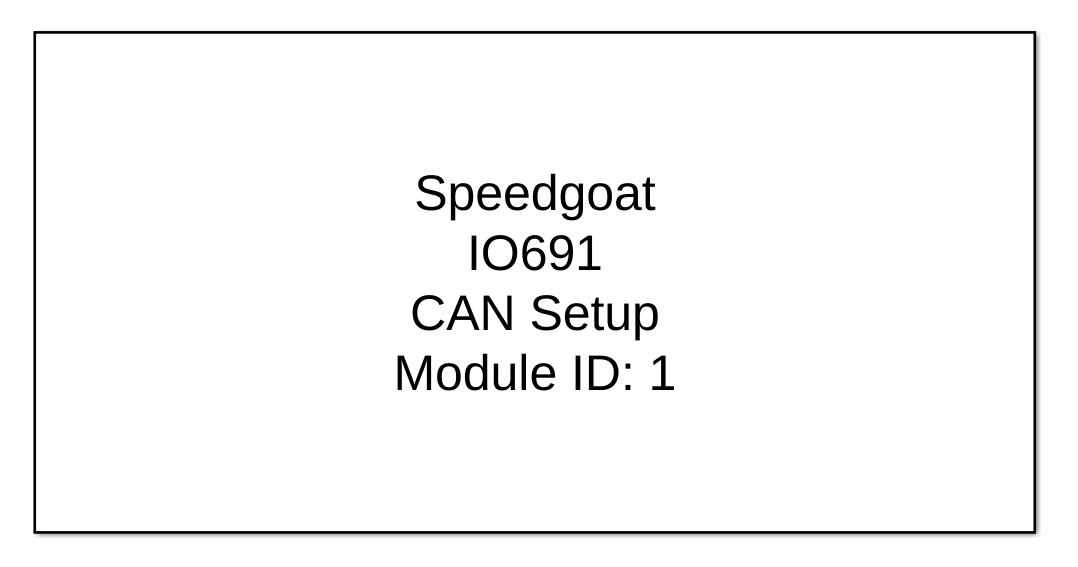
\includegraphics[width=0.7\textwidth]{img/4_simulink/IO691.png}
		\caption{Simulink – Driver Block – I/O Module 691 \cite{speedgoat:IO691}}
		\label{IO691_Konfigurieren:img:Driver_Block}
	\end{center}
\end{figure}
\pagebreak[1]


Die \frqq Initialization\flqq- und \frqq Termination\flqq-CAN-Nachrichten können individuell angepasst werden. Im nachfolgenden Matlab-Skript (\ref{IO691_Konfigurieren:code:Driver_Block}) werden die Variablen \frqq initCAN\flqq\ und \frqq termCAN\flqq\ definiert.



\pagebreak[4]
\begin{lstlisting}[language=Matlab, caption={Initialization and Termination Structure} \cite{speedgoat:IO691:CAN_Message}\label{IO691_Konfigurieren:code:Driver_Block}]
% create Initialization structure
initCAN.Channel     = 1;
initCAN.Protocol    = 'CAN-FD';         % 'CAN' or 'CAN-FD'
initCAN.BRS         = 1;                % 0 or 1
initCAN.Type        = 'Standard';       % 'Standard' or 'Extended'
initCAN.Identifier  = 99;               % ID must be double
initCAN.Data        = [8 8 8 8 8 8 8 8];
initCAN.Pause       = 0.05;

% create Termination structure
termCAN.Channel     = 1;
termCAN.Protocol    = 'CAN-FD';         % 'CAN' or 'CAN-FD'
termCAN.BRS         = 1;                % 0 or 1
termCAN.Type        = 'Extended';       % 'Standard' or 'Extended'     
termCAN.Identifier  = double(0xFFF);    % ID must be double
termCAN.Data        = [1 1 1 1 1 1 1 1];
termCAN.Pause       = 0.05



 
\end{lstlisting}
\pagebreak[1]

Die Baudrate kann in zwei Kategorien unterteilt werden: \frqq Nominal Baud Rate\flqq\ und \frqq Data Baud Rate\flqq. Wenn im \frqq CAN Channels\flqq-Menü der Modus \frqq CAN FD\flqq\ ausgewählt wird, können beide Baudraten konfiguriert werden. Im Modus \frqq CAN HS\flqq\ ist die Einstellung der \frqq Nominal Baud Rate\flqq\ möglich. \\
Es können entweder die voreingestellten Baudraten verwendet oder eigene Werte über ein Array [BRP, SJW, TSEG1, TSEG2] konfiguriert werden, deren Elemente im Folgenden kurz erläutert werden, siehe Tabelle \ref{IO691_Konfigurieren:tab:Baudraten}.

\pagebreak[1]
\begin{table}[!ht]
	\centering
	\caption{Simulink – Baudraten Parameter }
	\label{IO691_Konfigurieren:tab:Baudraten}
	\begin{tabular}{ll}
		\hline
		\multicolumn{1}{c}{\textbf{Abkürzung}} & \multicolumn{1}{c}{\textbf{Bedeutung}} \\ \hline
		\multicolumn{1}{l|}{BRP}               & Bit Rate Prescaler                     \\
		\multicolumn{1}{l|}{SJW}               & Synchronization Jump Width             \\
		\multicolumn{1}{l|}{TSEG1}             & Time Segment 1                         \\
		\multicolumn{1}{l|}{TSEG2}             & Time Segment 2                         \\ \hline
	\end{tabular}
\end{table}
\pagebreak[1]



Die sogenannte \frqq CAN Nominal Bit Time\flqq, wie in Abbildung \ref{IO691_Konfigurieren:img:Baudrate} dargestellt, besteht aus vier Segmenten: dem \frqq Sync Segment\flqq, dem \frqq Propagation Segment\flqq, dem \frqq\ Phase Buffer Segment 1\flqq\ und dem \frqq Phase Buffer Segment 2\flqq.
Das \frqq Sync Segment\flqq\ dient zur Synchronisation der Knoten auf dem Bus und hat eine Länge von genau einem Zeitquantum.
Im \frqq Propagation Segment\flqq\ werden die physikalischen Verzögerungen im Busnetzwerk ausgeglichen \cite[1]{microchip:CANModule}.\\
Im \frqq Phase Buffer Segment 1\flqq\ werden positive Phasenfehler kompensiert, und das Segment kann während der Resynchronisation verlängert werden. Im \frqq Phase Buffer Segment 2\flqq\ hingegen werden negative Phasenfehler kompensiert, und das Segment kann während der Resynchronisation verkürzt werden.\\ \ \\



Der \frqq BRP\flqq\ ist ein Parameter, der das Zeitquant $t_q$ festlegt siehe Gleichung \ref{eq:tq}.
Der \frqq SJW\flqq\ ist ein Parameter, der die Länge von \frqq TSEG1\flqq\ verlängern und die Länge von \frqq TSEG2\flqq\ verkürzen kann, um die Synchronisation zwischen den Knoten zu gewährleisten, dabei darf \frqq SJW\flqq\ kleiner gleich \frqq TSEG2\flqq\ sein \cite{speedgoat:IO691:CAN_Message}.

Der Sample Point (SP) ist der Punkt innerhalb eines CAN-Bits, an dem die tatsächliche Datenabtastung stattfindet. Dieser Punkt kann durch das Verhältnis zwischen \frqq TSEG1\flqq\ und \frqq TSEG2\flqq\ angepasst werden.

\pagebreak[1]
\begin{figure}[!ht]
	\begin{center}
		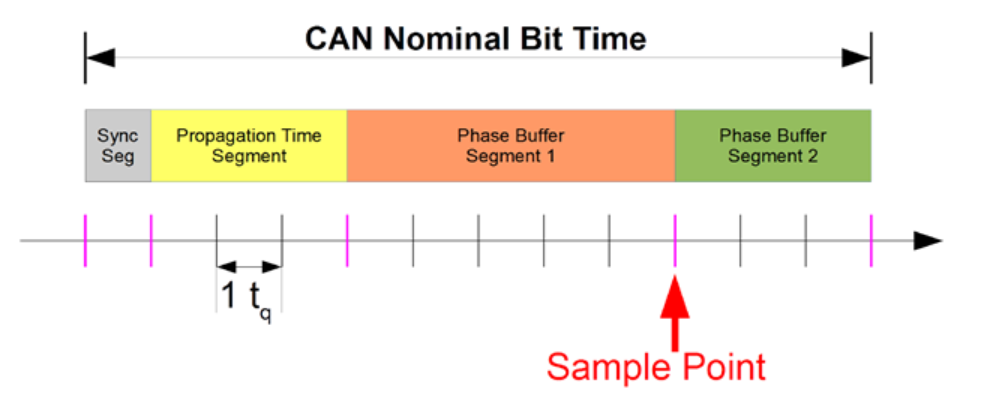
\includegraphics[width=1\textwidth]{img/4_simulink/IO691_Baudrate.png}
		\caption{Simulink – Baudrate – I/O Module 691 \cite{speedgoat:IO691:CAN_Message}}
		\label{IO691_Konfigurieren:img:Baudrate}
	\end{center}
\end{figure}
\pagebreak[1]

Mit den weiteren Gleichungen können die Zeiten innerhalb des \frqq CAN Nominal Bit Time\flqq\ ermittelt werden.
\begin{align}
	\label{eq:tq}
	t_{q}   & = \frac{BRP}{CAN_{Clk}} \\
	t_{BS1} & = t_{q}  \cdot TSEG1    \\
	t_{BS2} & = t_{q}  \cdot TSEG2
\end{align}

\begin{align}
	\begin{split}
		NominalBitTime & = t_{q} + t_{BS1} + t_{BS2}        \\
		               & = t_{q}  \cdot (1 + TSEG1 + TSEG2)
	\end{split}
\end{align}

\begin{align}
	CAN_{Baudrate} & = \frac{1}{NominalBitTime}
\end{align}

\begin{align}
	\begin{split}
		SP & = \frac{(1 + TSEG1)}{(1 + TSEG1 + TSEG2)} \\
		   & = \frac{(t_q + t_{BS1})}{NominalBitTime}
	\end{split}
\end{align}

Am CAN-Bus ist es wichtig, an beiden Enden Abschlusswiderstände von 120 $\Omega$ zu installieren. Diese Widerstände verhindern Reflexionen von Signalen, die auf der Leitung entstehen können, wenn die Impedanz des Busses nicht korrekt abgestimmt ist.\\
Reflexionen können das ursprüngliche Signal beeinträchtigen und zu Fehlern in der Datenkommunikation führen. Die Abschlusswiderstände gewährleisten eine angepasste Impedanz und minimieren somit die Wahrscheinlichkeit von Signalreflexionen \cite{speedgoat:IO691:CAN_Message}.
